\chapter{Comandi di base}
\section{Notazione}
Nel sorgente, lasciare una riga di spazio crea un nuovo capoverso. Andare a capo normalmente invece è come continuare sulla stessa riga. Per andare a capo uso \verb|\\|
Ecco le notazioni particolari
\begin{enumerate}
	\item \verb|^| Indica gli esponenti
	\item \_ Indica i pedici
	\item \% Indica i commenti
	\item \$ \$ Racchiude le formule matematiche
	\item Il comando \verb|\|verb restituisce ciò che è contenuto tra i caratteri | |
\end{enumerate}

\section{Formattazione}
\begin{enumerate}
	\item \verb|\|textbf\{\} grassetto
	\item \verb|\|underline\{\} sottolineato
	\item \verb|\|textit\{\} corsivo
	\item \verb|\|textsc\{\} maiuscoletto
	\item \verb|\|dots\{\} crea dei puntini di sospensione, mentre omissis crea puntini tra parentesi quadre
	\item \verb|\\| Forza ad andare a capo. Lasciare una riga bianca nel sorgente crea il nuovo paragrafo. Andare a 		capo nel sorgente non serve a nulla
	\item \verb|\|newpage inserisce comincia una nuova pagina
	\item posso usare \verb|\|small, \verb|\|large, \verb|\|huge seguiti da \{contenuto\} per modificare la dimensione del testo
	\item per allineare testo a destra/sinistra/centro uso \verb|\|begin\{flushleft/flushright/center\} 
\textit{quellochemipare} \verb|\|end\{flushleft/flushright/center\}
	\item per scrivere su più colonne uso \verb|\|begin\{multicols\}\{numerocolonne\} 
\textit{quellochemipare} \verb|\|end\{multicols\}
\end{enumerate}

\section{Elenchi}
Per creare elenchi numerati uso la sequenza di comandi:\\
{\itshape
\verb|\|begin\{enumerate\} \\
\verb|\|item primo \\
\verb|\|item secondo \\
\verb|\|item terzo \\
\verb|\|end\{enumerate\}}

Se voglio l'elenco senza numeri uso \textit{itemsize} al posto che \textit{enumerate}.
Posso anche usare \textit{description} e specificare dopo item, tra parentesi [ ] il nome dell'item per renderlo in grassetto e senza puntini. Se annido elenchi \textit{itemsize}, quelli più interni saranno caratterizzati da -.

\section{Tabelle}
Per creare una tabella uso i comandi\\
{\itshape
\verb|\|begin\{table\}\\
\verb|\|centering\\
\verb|\|begin\{tabular\}\{unaletterapercolonna\}\\
\verb|\|toprule\\
Nomecolonna \& Nomecolonna2 \& Nomecolonna3 \verb|\\| \\
\verb|\|midrule \\
elemento1 \& elemento2 \& elemento3 \verb|\\| \\
elemento1 \& elemento2 \& elemento3 \verb|\\| \\
elemento1 \& elemento2 \& elemento3 \verb|\\| \\
\verb|\|bottomrule \\
\verb|\|end\{tabular\} \\
\verb|\|end\{table\}} \\

Sostituendo tabular con array al posto di table creo una tabella matematica per formule. Specificando tra graffe 1 lettera per colonna, posso scegliere come giustificare il testo di ogni colonna. Posso usare \verb|\|caption\{nomedellatabella\} per dare un nome, oppure \verb|\|label{riferimento} per dare un riferimento richiamabile nel documento.

\begin{table}
\centering
\begin{tabular}{ll}
\toprule
Lettera & Effetto \\
\midrule
l & Allinea il contenuto della cella a sinistra \\
c & Centra il contenuto della cella \\
r & Allinea il contenuto della cella a destra \\
\bottomrule
\end{tabular}
\caption{Tabella bella bella}
\end{table}

\section{Personalizzazione}
Per colorare le parole uso la funzione \verb|\|textcolor\{colore\}\{quellochevoglio\}.\\
Per invece racchiudere in un box colorato pieno uso \verb|\|colorbox\{colore\}\{testo\}.\\
Per richiudere in un box liscio uso \verb|\|begin{tcolorbox} e \verb|\|end{tcolorbox}.\\

\textcolor{red}{ciao in rosso} \\
\colorbox{red}{ciao nel quadretto} \\
\begin{tcolorbox}
qui invece creo un quadretto
\end{tcolorbox}

\chapter{Matematica}
\section{Formule semplici}
Si racchiude la formula tra simboli \$\$
\section{Formule non numerate}
Si inizia la formula con \verb|\[| si scrive la formula e si conclude con \verb|\]|
\section{Formule numerate}
Si racchiude la formula tra \verb|\|begin\{equation\} e \verb|\|label\{nomeformula\}\verb|\|end\{equation\}\\
Per farvi riferimento si usa \verb|\|eqref\{nomeformula\}
\section{Funzioni}
\verb|\|frac\{primotermine\}\{secondotermine\} permette di scrivere una frazione.\\
\verb|\|sqrt\{termine\} restituisce la radice quadrata.\\
Il comando \verb|\[\|underbrace\{equazione\}\_\{scrivi quello che vuoi\} \verb|\]|permette di aggiungere un commento alla formula scritta.\\
Il comando \verb|\|\verb|int_margineinferiore^margineesuperiore{variabile \,dx}| \\permette di scrivere integrali.\\
La derivata si indica con un apice dopo il nome della variabile.\\
Il limite si scrive \verb|\lim_{x \to valoreacuitendex}funzione|.\\
Il comando \verb|sum_{i = 1}^{n}| può essere sfruttato per scrivere sommatorie.\\
Il comando \verb|\|dot/vec/hat/tilde/bar\{quellochevuoi\} pone una notazione sopra la variabile.\\
Il comando \verb|\|quad produce uno spazio nella formula.\\
I termini \verb|\|lvert e \verb|\|rvert racchiudono i valori assoluti.\\
Posso ingrandire le parentesi con \verb|\|bigr \verb|\|Bigr \verb|\|biggr \verb|\|Biggr per quelle di destra e con l al posto di r per quelle di sinistra.\\

\begin{figure}[H]
\centering
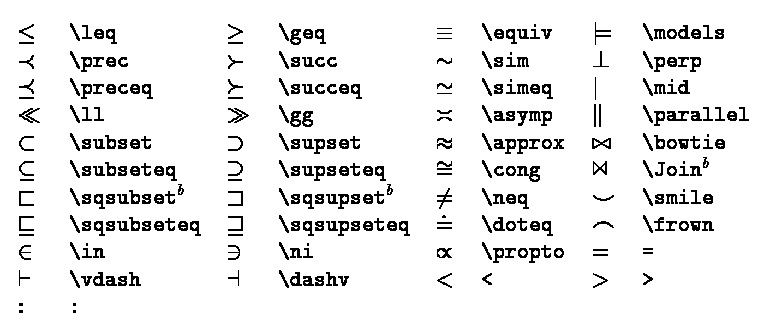
\includegraphics[scale=0.6]{t3}
\end{figure}

\begin{figure}[H]
\centering
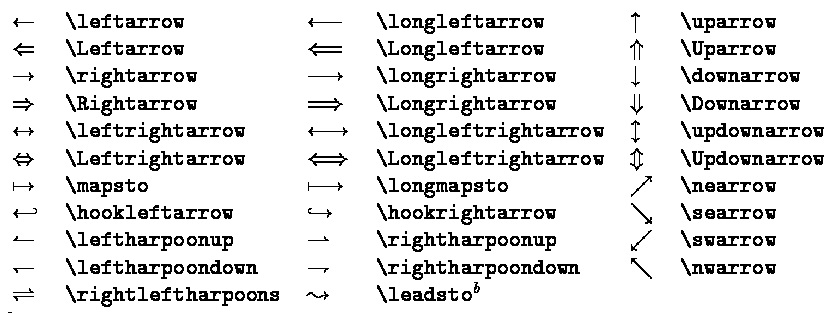
\includegraphics[scale=0.6]{t5}
\end{figure}

\section{Esempi}
Il quadrato di lato $\hat{l}$ è $A=l^2$

\begin{equation}f(x)=x^2+\frac{\sqrt{x^\frac{4}{3}}}{11x}\label{primaformula}\end{equation}
La formula \eqref{primaformula} è una semplice equazione.\\
Ecco ora un esempio di formula commentata:
\[
\underbrace{y}_{variabile\ dipendente}=\underbrace{4x+6}_{variabile\ indipendente}
\]
Ecco un esempio di integrale:
\[
\int_a^b{x\,dx}
\]
Ecco un esempio di limite:
\[
\lim_{x\to 0}
\frac{\sin x}{x}=1 
\]

\chapter{Figure}
\section{Inserire Figure}
\begin{figure}[H]
\centering
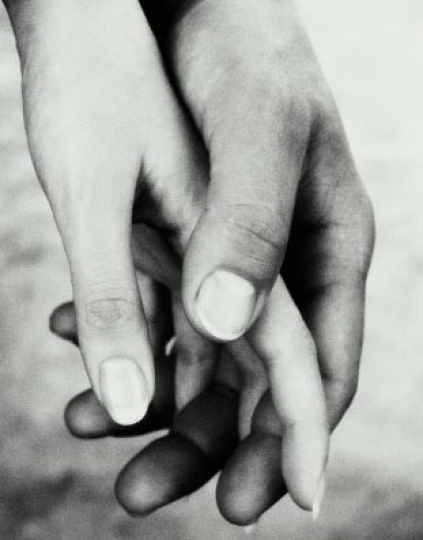
\includegraphics[scale=0.15]{mani}
\caption{mani che si stringono}
\label{fi}
\end{figure}

Posso inserire immagini con il comado\\
\verb|\|begin\{figure\}[H]\\
\verb|\|centering\\
\verb|\|includegraphics[parametri]\{nomeimmagine\}\\
\verb|\|end\{figure\}\\

Con \verb|\|caption\verb|{nomefigura}| fornisco il nome alla figura, mentre con \verb|\label{nomeimmagine}| creo un link di rierimento per essere richiamato nel testo.\\
Posso inserire diversi parametri con nome=valore separati da virgole tra le quadre, eccone alcuni:

\begin{table}
\centering
\begin{tabular}{ll}
\toprule
Parametro & Effetto \\
\midrule
width & imposta una larghezza massima \\
heigth & imposta un'altezza massima \\
scale & scala l'immagine \\
angle & Ruota l'immagine \\
\bottomrule
\end{tabular}
\caption{Tabella dei parametri}
\end{table}

\chapter{Riferimenti}
\section{Assegnazione nome}
Per assegnare un nome ad un oggetto, nome a cui poi fare riferimento, uso \verb|\label{nome}|
\section{Creazione Riferimento}
Per riferirsi ad un oggetto precedentemente nominato, uso \verb|\ref{nomeoggetto}|\\
Per riferirsi alla pagina dell'oggetto uso \verb|\pageref{nomeoggetto}|
\section{Esempio}
Faccio riferimento alla Figura \ref{fi} alla pagnia \pageref{fi}

\chapter{Documento da più file}
\section{Creazione}
Creo un file main nel quale includo i pacchetti, apro il documento, setto titolo e autore e creo l'indice. Dopodiche inserisco con \verb|\input{nomefile}| i file in cui sono contenuti i capitoli e chiudo il documento

N.B. nei vari files con i capitoli, inizio direttamente con \verb|\chapter{nomecapitolo}|, senza aprire prima il documento.

\chapter{Codice}
\section{Creazione}
Per scrivere codice devo prima inserire nell'header il corretto lstset, proprio di ogni lingagguio.
Poi basta inserire il codice racchiuso tra due \verb|\begin{Java}| e \verb|\end{Java}|
\section{Esempio}
\begin{Java}
// Hello.java
import javax.swing.JApplet;
import java.awt.Graphics;

public class Hello extends JApplet {
    public void paintComponent(Graphics g) {
        g.drawString("Hello, world!", 65, 95);
    }    
}
\end{Java}